\begin{apendicesenv}

\partapendices

\chapter{Termo de Abertura do Projeto}

\subsection{Objetivos deste documento}

Mesmo já havendo um consenso de ideia geral sobre o projeto, o TAP vem para autorizar formalmente o seu desenvolvimento, seja para as fases seguintes de planejamento, seja para construção efetiva da proposta. Ele também auxilia na definição de entregas por meio da EAP, no levantamento de requisitos, premissas e restrições, além de dar o grande suporte para o resto do planejamento, custo, riscos, tempo, escopo etc.

Elaborado este documento, o gerente de projetos tem a autorização, o poder e a base para o gerenciar corretamente todos os recursos disponíveis e otimizar seu planejamento durante o desenvolvimento do produto. Não deve ser esquecido que este documento deve ser descrito de forma que forneça suporte suficiente na aceitação ou não do projeto.


\subsection{Descrição do Projeto}

O projeto é uma máquina automática que auxilia no processo de reciclagem de garrafas. A ideia central é a de que o usuário insira garrafas de vidro ou plástico e seja bonificado por essa ação, onde tal, possa ser desconto em supermecados e estes dados serão mantidos por um aplicativo com contas individuais. A máquina deverá realizar a separação e validação (material, tamanho e peso) automática dos objetos inseridos, guardando a garrfas de vidro sem quebrá-las, triturando as de plástico e rejeitando qualquer outro tipo de inserção.

\subsection{Justificativa do Projeto}

A poluição global é um tema que visivelmente está sempre em discussão na mídia e nos governos por seu grande potência destrutivo. Dois dos grandes tipos de poluição que podem ser comentadas neste projeto são as de solo e do mar, sendo o motivo desta escolha comentado mais a frente, e é evidente que se sabe que o causador dessa agressão a esses dois tipos é o grande volume de material industrial criado pelo ser humano. Buscando minimizar esse problema, são realizadas diversas ações de reciclagem e conscientização ao redor do globo, sendo assim, este projeto vem com o intuito de criar um produto que motive estes dois fatores.

Para o desenvolvimento de um protótipo foram escolhidos dois tipos de materiais a serem coletados a partir das informações a seguir. O primeiro foi o plástico, pois segundo o site Ecycle, pesquisadores da The University of  Western Australia e da CSIRO Wealth from Oceans Flagship realizaram um estudo no mar australiano e concluíram que a cada quilômetro quadrado de água de sua superfície está contaminado por cerca de quatro mil pequenos fragmentos de plástico. Segundo o site da Globo, até 2015 tinham sido produzidos cerca de 6,3 bilhões de toneladas de resíduos plásticos e 79\% deste montante se encontra em aterros ou na natureza. Segundo o site Meio Ambiente Cultura Mix, sacolas plásticas e garrafas PETs são os maiores vilões da natureza pelo tempo de decomposição e pelo consumo destes materiais por animais. E o segundo foi o vidro pelo alto consumo de produtos mantidas em recipientes feitos deste material, o vidro pode causar queimadas na natureza por potencializar os raios solares e animais podem morrer ao ingerir pedaços cortantes. Portanto, serão dois materiais que causarão um grande impacto de projeto e eles estão diretamente ligados às poluições marítimas e de solo.

Outro fator que justifica a proposta deste projeto, são os impactos positivos para os usuários, que poderão receber créditos pela sua ação, empresas de reciclagem, que terão economia de armazenamento e manuseio, o governo, que terá seu nome em um projeto de apoio ambiental, os mercados, que poderão atrair mais clientes com promoções por conta da máquina e empresas geradoras dos resíduos já que pela lei nacional, elas são responsáveis pelo seus resíduos sólidos.

\subsection{Objetivos do Projeto}

O máquina tem como objetivos principais o incetivo a reciclagem por meio de um sistema de bonificações, o auxílio a coleta de material para as empresas de reciclagem e auxílio às empresas geradoras de resíduos sólidos já que elas são responsáveis pelo o que produz.

\subsection{Critérios de sucesso do projeto}

Tomando como referência o contexto de implantação do produto, os critérios de sucesso do projeto envolvem a dedicação máxima e estudo contínuo da equipe em seus subsistemas já que em sua maioria não se há investimento e nem experiência de trabalho. Rigorosa adesão ao planejamento e gerenciamento do projeto. Alcance dos requisitos levantados e integração completa.

\subsection{Estrutura Analítica do Projeto}

\begin{figure}[!ht]
	\centering
		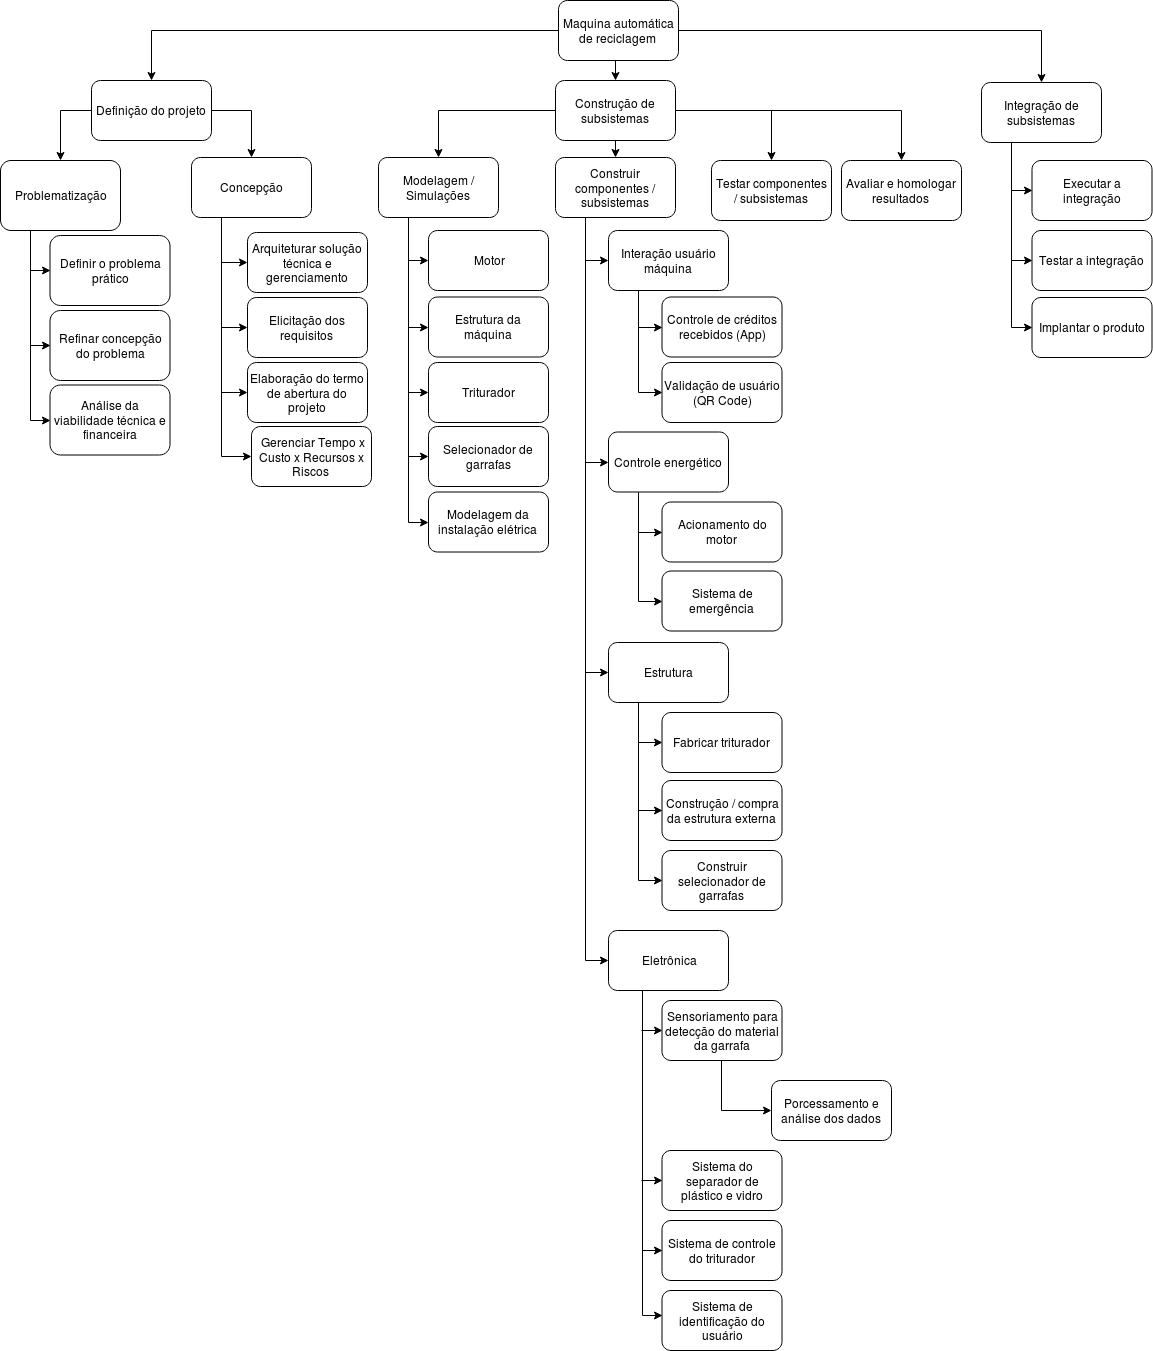
\includegraphics[scale=0.4]{figuras/eap}
	\caption{Estrutua Analítica do Projeto.}
\end{figure}

A EAP deste projeto está divida com base nas entregas definidas pelos orientadores. Como em todo projeto que se preze, o desenvolvimento do produto se sustenta na definição de um problema, elaboração de uma solução, construção do produto da solução e implantação e teste deste produto, logo abaixo estão descritos cada tópico da estrutura analítica voltados às necessidades de acompanhamento e gerência dos subsistemas deste projeto.

\begin{itemize}
    \item \textbf{Definição do projeto}
        Todo novo desenvolvimento de produto se inicia com a definição completa e planejada de um escopo geral e validado. Para começar, de forma geral, não seria viável a elaboração de um produto que não se resolve nenhum problema, sendo assim, é interessante a fase de definição ser divida na \textbf{Problematização} e \textbf{Concepção} baseada no ideia levantada.
        \begin{itemize}
            \item \textbf{Problematização}
                Essa fase envolve a aplicação de brainstormings para que o grupo possa avaliar o que há de problemas baseados na ideia central de projeto, para que assim, sejam anotados de forma planejada alguma de suas soluções que estejam ao alcance às áreas de conhecimento dos cursos da FGA. Em seguida, o problema deve ser refinado, de forma, que forneça base para a concepção completa e compreensível do escopo geral do produto que no caso é a solução proposta e para a análise da viabilidade técnica e financeira.
            \item \textbf{Concepção}
                Tendo sido levantada a ideia geral do projeto, aqui devem ser feitas os detalhamentos da arquitetura básica da solução, dos objetivos, regras de negócio e planejamento.
        \end{itemize}
    
    \item \textbf{Construção de Subsistemas}
        Após concretizado a definição do projeto, é o momento de iniciar o processo de desenvolvimento da máquina. Procurando facilitar a visão geral e organização, este processo foi divido em 4 atividades chaves:
        \begin{itemize}
            \item \textbf{Modelagem / Simulações}
                Uso do CAD, realização de cálculos diversos, uso de ferramentas de modelagem e geração de modelos de protótipos.
            \item \textbf{Construir componentes / Subsistemas}
                O sistema total do projeto foi dividido em 4 subsistemas com base nas áreas das engenharias com o intuito de otimizar a produtividade desacoplando as áreas. Nesta fase que acontece a construção real da máquina.
            \item \textbf{Testar componentes / Subsistemas}
                Fase de aplicação de plano de testes do componentes dentro dos subsistemas.
            \item \textbf{Avaliar e homologar resultados}
                Finalizado os testes, este é o momento de avaliar os resultados para levantamento do que deve ser otimizado afim de adaptar os componentes à atividade de integração. 
        \end{itemize}

    \item \textbf{Integração de Subsistemas}
        Esta em tese é a atividade mais complexa e que se tem um histórico alto de falhas, sendo assim, é necessário uma ótima preparação antecipada.
\end{itemize}

\subsection{Principais requisitos das principais entregas/produtos}

\begin{itemize}
    \item{Armazenamento de garrafas de plástico e vidro}
    \item{Armazenamento separado dos tipos de material}
    \item{Triturar as garrafas de plástico}
    \item{Armazenar em intacta as garrafas de vidro}
    \item{Bonificar os usuários por cada garrafa}
    \item{Manter dados do usuário em um aplicativo}
\end{itemize}

\subsection{Marcos}

\begin{table}[htp]
    \centering
    \caption{Marcos}
    \label{my-label}
    \begin{tabular}{|p{0.25\linewidth}|p{0.65\linewidth}|p{0.15\linewidth}|}
    \hline
    \multicolumn{1}{|c|}{\textbf{Fase}} & \multicolumn{1}{c|}{\textbf{Marcos}} & \multicolumn{1}{c|}{\textbf{Previsão}} \\ \hline
    Iniciação & Projeto Aprovado & 28/03/2018 \\ \hline
    Planejamento & Plano de Gerenciamento de Projetos Aprovado & 28/03/2018 \\ \hline
     & Linhas de Base de Custos, Prazo e Escopos Salvas & 28/03/2018 \\ \hline
    Execução, Monitoramento e Controle & Desenvolvimento dos subsistemas & 16/05/2018 \\ \hline
    Encerramento & Integração & 26/05/2018 \\ \hline
     & Testes & 06/06/2018 \\ \hline
     & Projeto Entregue & 22/06/2018 \\ \hline
    \end{tabular}
\end{table}

\subsection{Partes interessadas do projeto}

É preferível pela equipe de trabalho que as partes interessadas sejam divididas em dois grupos, o primeiro são os reais interessados dentro do contexto e escopo atual que é a matéria do curso, e o segundo são os possíveis interessados em uma possível implantação comercial deste produto.

\subsubsection{Partes interessadas em cenário acadêmico}

\begin{table}[htp]
    \centering
    \caption{Cenário acadêmico}
    \label{my-label}
    \begin{tabular}{|p{0.35\linewidth}|p{0.35\linewidth}|p{0.35\linewidth}|}
    \hline
    \multicolumn{1}{|c|}{\textbf{Nome}} & \multicolumn{1}{c|}{\textbf{Função}} & \multicolumn{1}{c|}{\textbf{Interesse}} \\ \hline
    Professores da Matéria Projeto Integrador II do Campus de Engenharias da UnB & Orientar e avaliar os alunos no desenvolvimento do projeto & Orientar e avaliar os alunos no desenvolvimento do projetoSaber se os alunos da matéria estão hábeis a serem egressos da universidade \\ \hline
    Alunos da Matéria Projeto Integrador II do Campus de Engenharias da UnB & Desenvolver o projeto & Receber feedback da qualidade do projeto e da qualidade de trabalho. \\ \hline
    \end{tabular}
\end{table}

\subsubsection{Partes interessadas em cenário de mercado}

\begin{table}[htp]
    \centering
    \caption{Cenário de mercado}
    \label{my-label}
    \begin{tabular}{|p{0.35\linewidth}|p{0.35\linewidth}|p{0.35\linewidth}|}
    \hline
    \multicolumn{1}{|c|}{\textbf{Nome}} & \multicolumn{1}{c|}{\textbf{Função}} & \multicolumn{1}{c|}{\textbf{Interesse}} \\ \hline
    Clientes de supermercado & Utilizar a máquina & Ser bonificado pelo uso \\ \hline
    Empresas de reciclagem & Buscar e reciclar o material armazenado pela máquina & Economizar em manuseio e transporte do material \\ \hline
    Empresas geradoras de Resíduos Sólidos & Gerar os resíduos sólidos & Economia na gerência de seus resíduos \\ \hline
    Governo & Aplicar e apoiar serviços deste cunho & Ter um projeto deste cunho vinculado ao seu nome \\ \hline
    \end{tabular}
\end{table}

\subsubsection{Restrições}
O projeto está restrito a ser um protótipo por conta do tempo de projeto (um semestre letivo), inexperiência da equipe (primeiro experiência de projeto em conjunto com o intuito de integração de várias áreas de engenharia) e falta de orçamento (máximo de R\$ 3.900,00).

\subsubsection{Premissas}
\begin{itemize}
    \item{Os testes de uso serão realizados apenas com os integrantes do time de desenvolvimento}
    \item{O tempo de trituração poderá ser avaliado apenas durante o desenvolvimento}
    \item{A prova de integração entre o aplicativo e a máquina será via display simples}
    \item{A disponibilidade de horário comum da equipe é apenas no horário de aula}
    \item{Não haverá recursos vindos de fora da equipe}
\end{itemize}

\subsubsection{Riscos}
Os principais riscos levantados inicialmente são:
\begin{itemize}
    \item{Inexperiência dos membros da equipe com ferramentas e tecnologias a serem utilizadas}
    \item{Peças que demoram a ser obtidas estarem com defeito}
    \item{Aceito não gratuito a equipamentos de alto curto realmente necessários}
    \item{Falta de espaço para construção da estrutura}
    \item{Falha na integração}
\end{itemize}

\subsubsection{Orçamento do Projeto}
\begin{table}[htp]
    \centering
    \caption{Orçamento}
    \label{orcamento}
    \begin{tabular}{|l|l|}
    \hline
    Ambiente do Usuário & R\$ 00,00 \\ \hline
    Sistema de Controle de Energia e Segurança & R\$ 1370,00 \\ \hline
    Estrutura & R\$ - \\ \hline
    Sistema Eletrônico & R\$ 520,00 \\ \hline
    \multicolumn{2}{|c|}{\textbf{R\$ 1.890,00}} \\ \hline
    \end{tabular}
\end{table}
    

\chapter{Plano de Gerenciamento de Riscos}

\end{apendicesenv}
